\section{Différents algorithmes de détection}

\subsection{Principe du CA-CFAR (cell-averaging Constant False Alarm Rate)}

La détection CFAR "Constant False Alarm Rate" fait référence à
une forme classique d'algorithme adaptatif utilisée dans les radars pour isoler le signal retour d'une cible d'un bruit de fond important, de brouillage et d'interférences. Le principe de cet algorithme est de tester une cellule (Cell Under Test : CUT) afin de savoir si une cible est présente ou s'il s'agit uniquement de bruit ou d'interférence. Pour cela, on estime le niveau de bruit de fond à l'aide des cellules adjacentes à la CUT, ces cellules sont appelées Cellules de Références (Reference Cells : RC). Pour éviter que les résultats soient faussés par la puissance reçue dans la CUT, on élimine du calcul les cellules immédiatement adjacentes (Guard Cells).Une cible est considérée présente dans la CUT si son signal est à la fois supérieur aux cellules adjacentes et au niveau de puissance moyen calculé. Voici un schéma explicatif des cellules de détection dans le cadre de la détection CFAR : 

\begin{figure}[h]
    \centering
    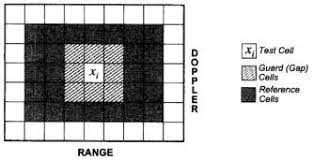
\includegraphics[width=0.6\textwidth]{src/rapport_complet/img/cellule_CFAR.jpg}
    \caption{Cellule de détection CFAR}
    \label{fig:image_radar_CFAR}
\end{figure}








\subsubsection{Estimation du bruit}

Le niveau du clutter (fouillis radar : échos parasites) est estimé par la moyenne arithmétique des échantillons dans la fenêtre de référence donnée par \cite{fstech_chapitre5_cfar}: 
\begin{equation}
{Q}_{\text{clutter}} = \frac{1}{M} \sum_{i=1}^{M} x_i
\end{equation}

\begin{description}
  \item[${Q}_{\text{clutter}}$ :] estimation du niveau moyen du clutter (ou du bruit de fond)
  \item[$M$ :] nombre total de cellules de référence
  \item[$x_i$ :] puissance mesurée dans la $i^{\text{ème}}$ cellule de référence
\end{description}

Si on considère la détection quadratique, la FDP (fonction de densité de probabilité) de la variable aléatoire à la sortie du détecteur, X, suit
la loi Exponentielle donnée par :
\begin{equation}
f_X(x) = \frac{1}{2\sigma^2} e^{-x / 2\sigma^2}, \quad x \ge 0
\end{equation}


\subsubsection{Calcul du seuil de détection}

Le seuil (seuil adaptatif) de détection correspond au niveau à partir duquel on estime qu'une cible est détectée. Il s'écrit comme : 
\begin{equation}
T = \alpha Q
\end{equation}

\subsubsection{Probabilité de fausse alarme et Probabilité de détection}

\paragraph{Probabilité de fausse alarme (\(P_{\text{fa}}\))}  
La probabilité de fausse alarme correspond à la probabilité qu'une mesure dépasse le seuil de détection alors qu'aucune cible n'est présente.  
Autrement dit, c'est la probabilité que le détecteur décide à tort qu'il y a une cible, alors que le signal observé provient uniquement du bruit.

\[
P_{\text{fa}} = P(X > T \,|\, H_0)
\]

où \( H_0 \) représente l'hypothèse \textit{« absence de cible »}.

\vspace{1em}

\paragraph{Probabilité de détection (\(P_{\text{d}}\))}  
La probabilité de détection correspond à la probabilité qu'une mesure dépasse le seuil de détection lorsqu'une cible est effectivement présente.  
C'est donc la probabilité que le détecteur prenne la bonne décision en présence d'un signal utile.

\[
P_{\text{d}} = P(X > T \,|\, H_1)
\]

où \( H_1 \) représente l'hypothèse \textit{« présence de cible »}.
